\documentclass[../main.tex]{subfiles}
\graphicspath{
    {"../img/"}
    {"img/"}
}

\begin{document}
Ulice w Warszawie to po prostu bardzo długa prosta po której poruszają się ciągłe samochody.
Żeby to tak działało, to można warunek ciągłości zapisać tak:
\[
    \rho_t + v_m\left( 1 - \frac{2\rho}{\rho_m} \right) \rho_x = 0,\quad v_m, \rho_m > 0
.\]
Przepisujemy do postaci
\[
    \frac{\partial q}{\partial \rho} \frac{\partial \rho}{\partial x} = v_m \left( 1 - \frac{2\rho}{\rho_m} \right) \frac{\partial \rho}{\partial x}
.\]
Dzielimy przez pochodą $\rho$
 \[
     \frac{\partial q}{\partial \rho} = v_m - \frac{2v_m}{\rho_m}\rho
.\]
No i wychodzi jak się scałkuje
\[
    q(\rho) = v_m \rho - \frac{v_m}{\rho_m}\rho^2 + c
.\]
Interpretacja stałych $\rho_m$ i $v_m$ - gęstość i prędkość maksymalna. One w ogóle zaczną się odpychać przy za dużej gęstości, bo jest ten minus przy $v_m$.
Zadajemy warunek początkowy
\begin{equation}
    \label{eqn:pocz}
    \rho\left( t=0, x \right) = \rho_m \theta(-x)
\end{equation}
\begin{pytanie}
    Jaka to sytuacja na drodze?
\end{pytanie}
\textbf{Odp.} No światła drogowe.

To teraz trzeba narysować charakterystyki.\\
Co to znaczy równanie ciągłości ale z nie-stałymi współczynnikami?
\[
    u(t,x(t)) = const \implies \frac{\partial u}{\partial t} + \frac{\partial u}{\partial x} \frac{\partial x}{\partial t} = 0 \implies \frac{\partial u}{\partial t} = - \frac{\partial u}{\partial x} \frac{dx}{dt}
.\]
Czyli dalej
\[
    -\frac{\partial u}{\partial x} \frac{dx}{dt} + \frac{\partial q(u)}{\partial x} = 0 \implies \frac{\partial q}{\partial u} = \frac{dx}{dt} \implies x(t) = \int q'(u)dt
.\]
Dla warunku \eqref{eqn:pocz}, wyglądać będzie jakoś tak\\
\[
    x(t) = q'(g(\xi))t + \xi = v_m\left( 1 - \frac{2\rho_m}{\rho_m} \right) t + \xi = -v_mt + \xi
.\]
\begin{figure}[h]
    \centering
    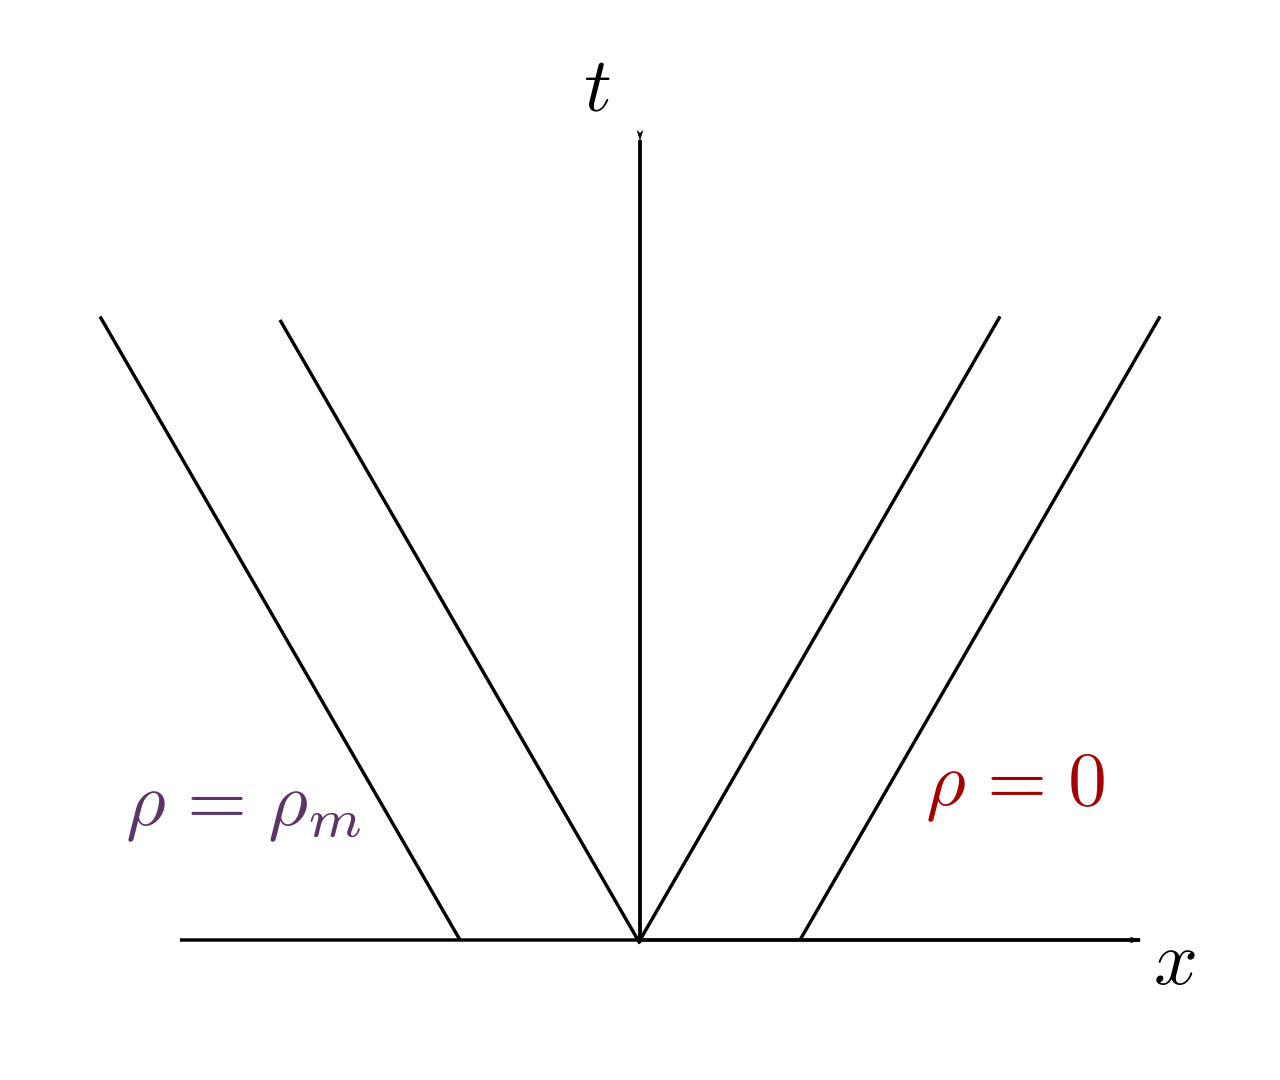
\includegraphics[width=0.4\textwidth]{swiatla-drogowe}
    \caption{Tak wyglądają nasze charakterystyki}
    \label{fig:swiatla-drogowe}
\end{figure}

\[
    s'(t) = \frac{q(0) - q(\rho_m)}{0 - \rho_m} = \frac{c - c - v_m\left( \rho_m - \rho_m \right) }{-\rho_m} = 0
.\]
No to mamy jedno fajne rozwiązanie.
A inne?
\[
    \rho(t,x) = \begin{cases}
        \rho_m & x <0\\
        0 & x > 0
    \end{cases}
.\]
\[
    q' = v_m (1-\frac{2\rho}{\rho_m})
.\]
\[
    \rho = - \frac{q' - v_m}{2v_m}\rho_m
.\]
\[
    R(\alpha) = \left( \frac{v_m - \alpha}{2v_m} \right) \rho_m
.\]
\[
    R\left( \frac{x-x_0}{t-x_0} \right)  = \frac{v_m - \frac{x}{t}}{2v_m} \rho_m = \rho(x,t)
.\]
\end{document}
